\chapter{Big Data tools}
\label{chap:chapter2}
In this chapter we will describe the tools used for implementing a working prototype based on Lambda architecture paradigm previously explained. The scope of this thesis is not to make a survey of modern technologies for big data and here we will give just an overview highlighting purpose and main features of each used tool. For a better understanding of these tools, the reader is invited to consult additional resources about them.
\section{Kafka}
Apache Kafka \cite{bib19} is a general purpose distributed publish-subscribe message system originally developed at Linkedin and then opensourced in 2011 and inserted in the Apache ecosystem. The architecture is composed by one or more servers, also known as \textit{brokers}, which rely on Apache Zookeeper for coordination.\\
The key abstraction in Kafka is a topic: \textit{producers} publish messages to a topic and \textit{consumers} subscribe to one or more topics. A single topic is composed by a set of partitions, distributed and replicated among all the brokers in the cluster. For each partition there is a master replica and a set of slaves. Since normally there are more partitions than brokers, a broker can play the role of master some partitions and the role of slave for others. For each partition are saved metadata about consumers positions, also called offsets. An offset represents a checkpoint for that consumer, messages before it are assumed to be correctly processed and the next time a consumer makes a fetch request, the broker will forward messages starting from the last offset. The consumer, anyway, is still able to reprocess already committed messages, for instance in response to a failover event.\\
\begin{figure}[h]
        \centering
        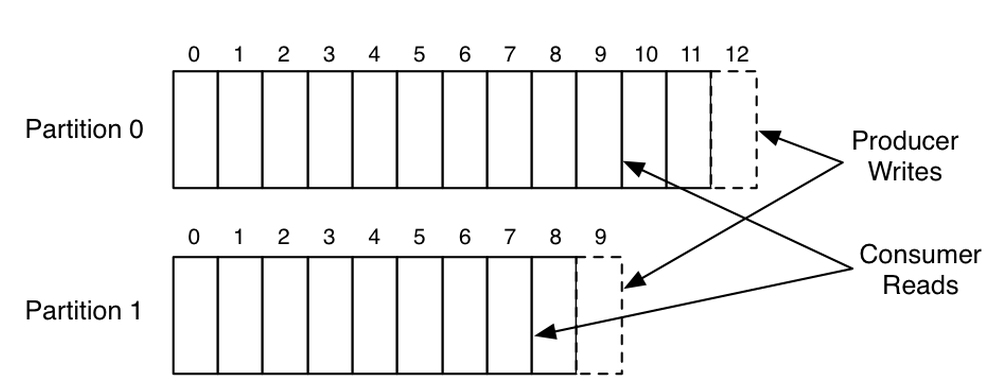
\includegraphics[width=12cm]{imgs/kafka-topic}
\caption[Kafka topic]{A 2-partitions topic with one producer and one consumer.\protect\footnotemark}
        \label{kafka-1}
\end{figure}
\footnotetext{https://engineering.linkedin.com/kafka/benchmarking-apache-kafka-2-million-writes-second-three-cheap-machines}

What it is interesting in Kafka is how messages are forwarded from the producer to the consumer through the brokers. Unlike other messaging systems which process  messages in-memory, Kafka does a strong usage of the filesystem: messages are immediately stored on filesystem and not deleted when read by a consumer but retained according to a configurable period. This avoid any kind of data loss for every committed message, even in case of brokers failure. The only information retained by brokers is the consumers positions across the topics. These information are generally stored on Zookeeper. \\
Kafka allows to implement either a \textit{queuing} or a \textit{publish-subscribe} logic introducing the abstraction of \textbf{consumer group}.
Each consumer labels itself with a  group name and is it responsible for reading from one or more partitions of a topic. Kafka ensures than no more than one consumer per group reads from a partition: if in the group there are more consumers than partitions, some of them will stay idle. In the opposite scenario, a consumer will read from more than one partition.
If all the consumers belong to the same group, then the system works as a queue, balancing the load across the consumer group. If all the consumers have different groups, then the system works as a standard publish-subscribe.\\
\begin{figure}[h]
        \centering
        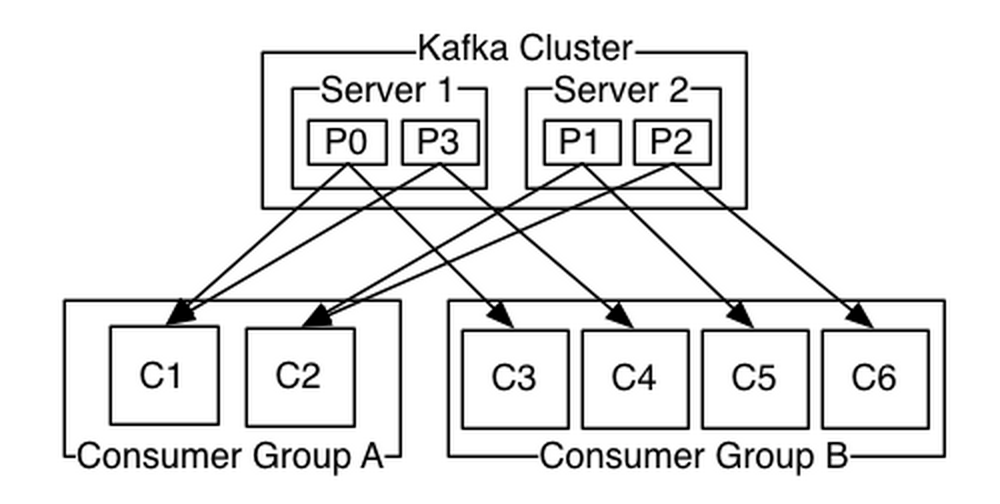
\includegraphics[width=12cm]{imgs/kafka-cgroup}
\caption[Kafka consumer group]{Two consumer groups read from a 4-partition topic.\protect\footnotemark}
        \label{kafka-2}
\end{figure}
\footnotetext{http://kafka.apache.org/documentation.html}

Having the concept of the consumer group implies a total order over the messages within each partition: the order on how are messages are read inside a partition is the same for every consumer who subscribed that partition.\\
As a conclusion, is worthy mention that Kafka implements by default a \textit{at-least-once} message semantic in the following way:
\begin{itemize}
\item Producer: when publishing a message and having a network error, the producer can't be sure if the message has been correctly committed to the broker.
\item Consumer: a message is said to be fully processed (from a broker perspective) only when its offset has been committed. The best the consumer can do is, read the message, process it and then commit the offset. If the consumer crashes  before committing the offset but after processing the message, the one taking over will process the same message.
\end{itemize}

\section{Hadoop}
\label{yarn}
Hadoop is an open-source suite for scalable fault-tolerant distributed computing written in Java. Based on Google's  \textit{Map-Reduce} \cite{bib25} approach, it was first developed in order to run MapReduce jobs for processing a web crawl. The rapid increase of popularity led to an abuse of the original computing paradigm exposed by Hadoop such as run heterogeneous task in a multi-tenant environment. In 2013, a second version of Hadoop, YARN \cite{bib24}, was released with the purpose of compensate the limitations of Hadoop first version, in primis decouple the programming model from the resource management layer and support a multi-tenancy job scheduler. 
\begin{figure}[h]
        \centering
        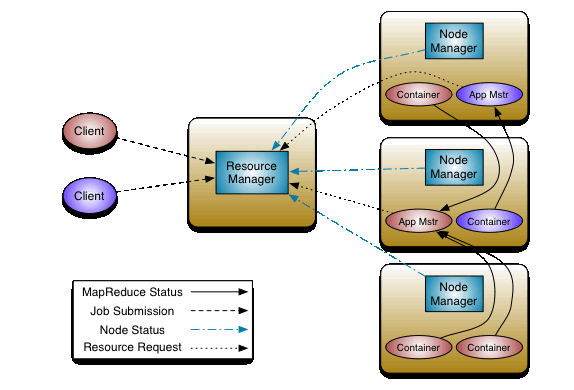
\includegraphics[width=12cm]{imgs/yarn-architecture}
\caption[YARN architecture]{YARN architecture\protect\footnotemark}
        \label{yarn-1}
\end{figure}
\footnotetext{http://hadoop.apache.org/docs/r2.7.0/hadoop-yarn/hadoop-yarn-site/YARN.html}
The architecture of YARN is composed by a global per-cluster \textit{Resource Manager (RM)} with duties of scheduling jobs submitted by clients and allocating resources when needed by the applications running on the cluster. Having a centralized coordinator enables scheduling properties of fairness, capacity and locality. The architecture is completed by one or more \textit{Node Managers (NM)} running on each slave node in the cluster. NMs are the workers daemons, in charge of monitoring the execution of the applications running on its node. Resources are spawned across running applications in form of \textit{containers}. A per-application daemon called \textit{Application Master (AM)} dynamically requests to the RM bundles of resources (containers) in order to execute the application it is responsible of. In this scenario, the RM is agnostic of the applications logics as it only replies to resources requests. MapReduce is now only a class of applications Hadoop YARN supports and several computation framework implementing different programming models has been adapted for being executed on top of YARN (Spark, Storm, Tez, Giraph and others).

\subsection{HDFS}
Hadoop distributed storage implementation is called HDFS (Hadoop Distributed File System). It is a highly efficient storage solution perfectly integrated with applications running on Hadoop, supporting the main operations of a normal filesystem and structured in a folder hierarchy. It is composed by a master/slave architecture with by one \textit{Namenode} and at least one \textit{Datanode}.
\begin{figure}[h]
        \centering
        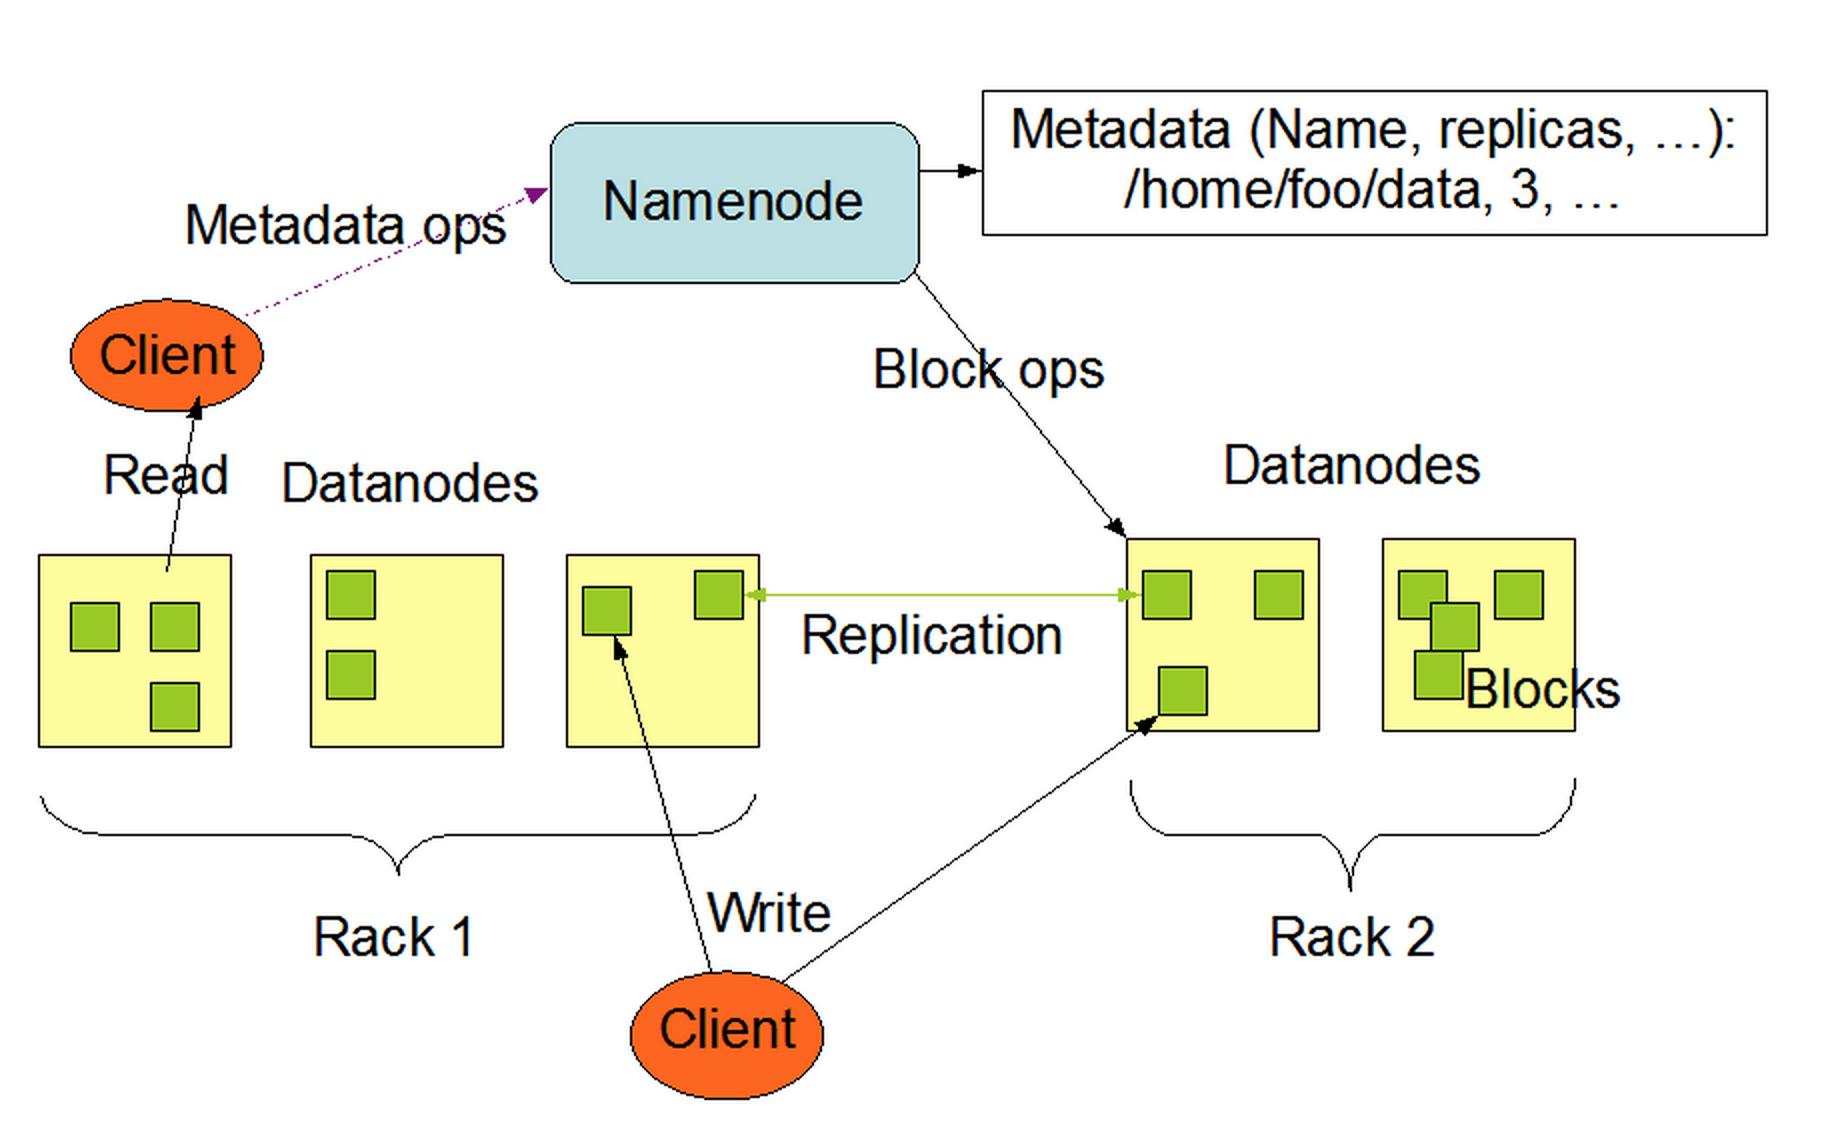
\includegraphics[width=12cm]{imgs/hdfs-architecture}
\caption[HDFS architecture]{HDFS architecture\protect\footnotemark}
        \label{hdfs-1}
\end{figure}
\footnotetext{http://hadoop.apache.org/docs/r2.7.0/hadoop-project-dist/hadoop-hdfs/HdfsDesign.html}
A Namenode holds the namespace of the filesystem, i.e. information about the structure of the filesystem and metadata about the distribution of the files over the datanodes, and listens for client requests such as writes or reads. Datanodes are the worker nodes: they store data and they serve the actual client requests, providing for data in case of read requests or allocating space in case of write requests. In this architecture, Namenode represents a single point of failure, the namespace is kept in memory by the Namenode and it case of its failure all data is compromise. There are several solutions to run HDFS in \textit{High Availablility (HA)} mode such a maintaining a \textit{StandBy} replica synchronized with the master through a network file system \cite{bib23}\\
A file in HDFS is split in several blocks according to its size (HDFS handles block of 128Mb by default), distributed and replicated across the Datanodes according to a per-file policy. The position of each blocks and their replicas are kept in Namenode's namespace. Having a block abstraction gives robustness and fail-tolerance to the storage system in case of Datanodes failure: client requests are normally redirected to the nearest healthy Datanode containing the required information.
\subsection{Oozie}
Apache oozie\cite{bib20} is a workflow scheduler for Hadoop. Each workflow is composed by a sequence of action executed in sequential mode, which means that an action can't be executed until the previous one ended. If configured with YARN resource negotiator, Oozie runs each job in a container context [\ref{yarn}].
Oozie workflow builds a DAG (direct acyclic graph) structure and is composed by a sequence of two possible type of \textit{nodes}:
\begin{itemize}
\item control flow: nodes that control the start, the end and the execution of the workflow without executing any concrete action. Example of this nodes are: start control node, end control node, kill control node, fork control node.
\item action: nodes that execute a task. The actions supported by the latest version (4.2.0 July 2015) are Map-Reduce, Pig, Java, Fs (filesystem), ssh, Spark	 
\end{itemize}
Jobs are scheduled by the server with a minimal granularity of minutes. It is possible to specify an input and an output directory where to read data needed to the job and where to store an eventual result. Moreover, the input and the output directories paths can be expressed in a dynamic way using time  expressions which are evaluated differently according to when the job is executed. All the configurations are submitted to the server using XML files containing information about the location of the application executables, directories paths, application arguments and frequency of the jobs. These configuration files are uploaded on HDFS for being accessible by any node in the cluster.

\section{Spark}
Apache Spark is a distributed framework for batch data processing. It is based on the same paradigm of Hadoop/Map-Reduce, where the computation is split across several nodes in the cluster (\textit{map}) and the final result is given by aggregating the intermediate ones (\textit{reduce}). Spark has been designed for the class of applications which need to iterate several times on the same dataset, such as machine learning and interactive analytics, allowing them to store intermediate data in memory instead of recompute it at every step. For these type of applications, it has been showed how spark outperforms a classic map-reduce paradigm by 10 times \cite{bib21}.\\
In order to be executed in a distributed mode, Spark needs a cluster manager for resources allocation across all the nodes. Spark provides its own standalone cluster manager even though YARN or Mesos can be used. The architecture is composed by a primary node called \textit{driver program} and a set of worker nodes running \textit{executor} threads. When an application is submitted to the cluster, the driver program spreads it across the worker nodes and schedules task to be run by each executor in an independent context (each executor runs its own JVM). In this way there is complete isolation between several applications running on the same cluster, the drawback is that executors belonging to different applications can't share data between themselves and also within the same application they need the support of the driver program for sharing data using special objects such as \textit{broadcast} and \textit{accumulator} variables.

\begin{figure}[h]
        \centering
        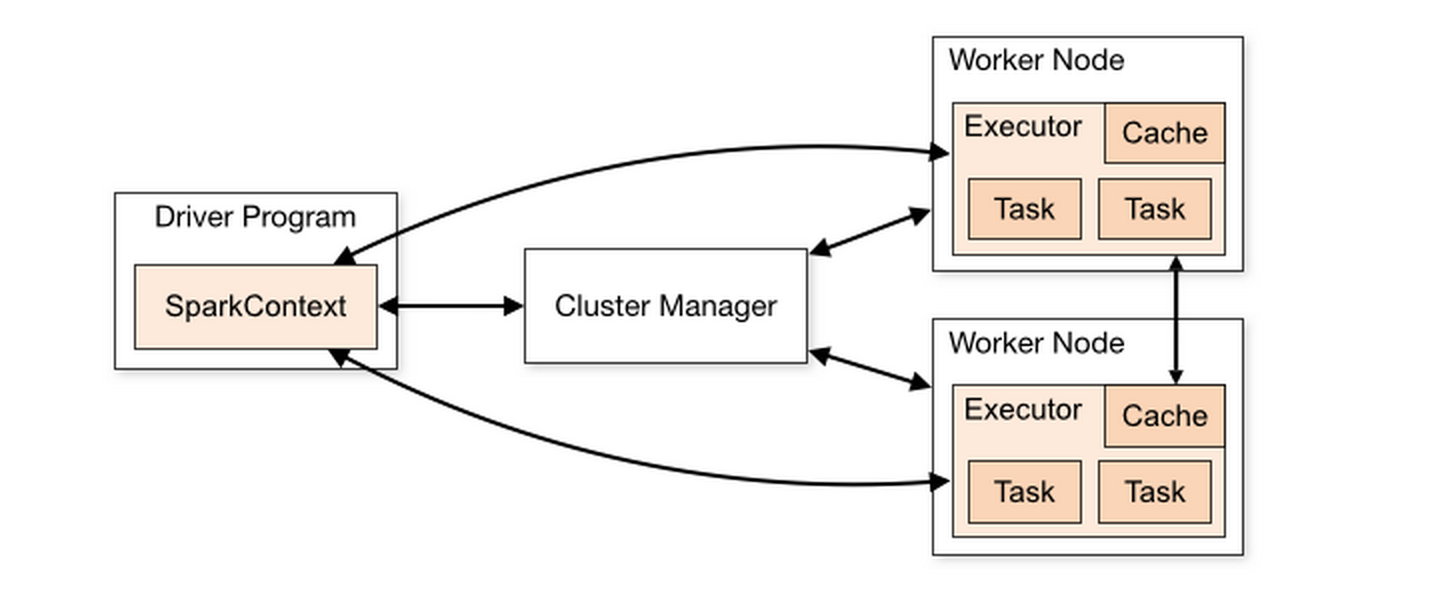
\includegraphics[width=12cm]{imgs/spark-architecture}
\caption[Spark cluster architecture]{Spark cluster architecture\protect\footnotemark}
        \label{spark-1}
\end{figure}
\footnotetext{https://spark.apache.org/docs/latest/cluster-overview.htmld}
The main concept around Spark is an abstraction over a physical dataset called \textit{RDD} \cite{bib8} (resilient distributed dataset). RDDs are read-only, fault-tolerant parallel data structures divided into one or more partitions across a set of machines. They can be created from physical files, parallelizing a collection of elements or modifying an existing RDD by applying a transformation (map, filter...) or an action (reduce, count...). RDD are lazy by nature, in the sense that the driver program keeps in memory the list of transformations needed to compute it rather than execute them at each step. Only when an action requires the RDD to be returned to the driver program, the list of transformations is applied. By default, each transformed RDD is re-calculated each time an action runs on it. It is possible however, to cache it in memory for faster successive accesses. This abstraction increases the robustness of the data model: in case of a partition failure, it can be reconstructed by applying the list of transformations and actions from the last RDD available in memory.

\section{Storm}
Apache Storm is a distributed real-time data processing framework created by Nathan Marz (the proposer of Lambda architecture). Storm considers the data as a stream of \textit{Tuple}, generated in special component called \textit{spouts} and processed by one or more \textit{bolts}.\\ Spouts and bolt can be combined in a direct graph structure called \textit{topology}. Each component (spout or bolt) can be replicated for load distribution. \\
A Storm cluster is composed by a master node and one or more worker nodes. The master node runs a process called \textit{Nimbus}: it handles applications submissions and it is responsible for distributing the code across the nodes, assigning tasks and checking for failures. The worker nodes run one or more processes called \textit{supervisors} in charge of communicating with the master and of executing worker processes.
\begin{figure}[h]
        \centering
        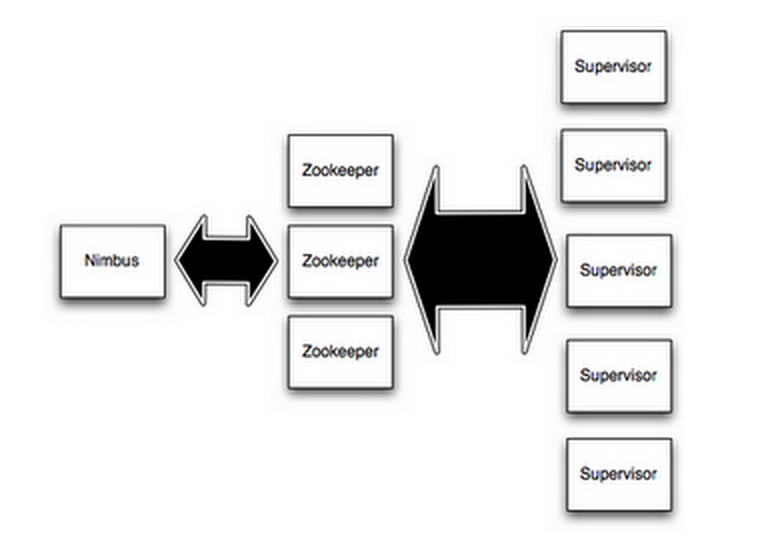
\includegraphics[width=10cm]{imgs/storm-architecture}
\caption[Storm cluster architecture]{Storm cluster architecture\protect\footnotemark}
        \label{storm-1}
\end{figure}
\footnotetext{https://storm.apache.org/documentation/Tutorial.html}
Within a worker process it is possible to run one or more \textit{executor} threads , each \textit{executor} finally runs one or more tasks, with are just parts of the topology belonging to the same component.
As stated before, the main abstraction in Storm the stream of Tuple. Data flows from a component to the next one according to a partition policy: data can be distributed in shuffle mode, by a key, towards a unique component or replicated. Each mode fulfils a different use case: for instance a key-partition (\textit{fields grouping}) is useful when we want to count the occurrences of a particular element in the data stream while a shuffle partition(\textit{shuffle grouping}) is a better approach when the same operation can be performed on each tuple, independently of the actual content of the tuple itself.\\
Storm guarantees by default a \textit{at-least-once} message processing semantic. A topology can be launched with acker components, responsible of ensuring that a tuple is successfully processed within a timeout. Storm keeps in memory a DAG for each tuple generated by a spout: each node in the DAG represents a component which is supposed to process the tuple and sends an ack on success. If the acker receives all the acks for a tuple then that tuple is said to be fully processed, otherwise the tuple is considered failed and the spout responsible for it should be able to regenerate it. In this way no data loss is guaranteed, but a tuple might be processed more than once. 

\section{Elasticsearch}

Elasticsearch is a distributed full-text search engine built on top of Apache Lucene. It provides a set of Rest API for documents indexing, querying and real-time analytics. In order to give a better understanding of how documents are organized inside a cluster, it is possible to compare Elasticsearch structure to a relational database where:
\begin{itemize}
\item a database is called \textit{index}
\item a table is called \textit{type}
\item a table row is a \textit{document} in JSON format
\item a table column is a \textit{field}
\end{itemize}
Elasticsearch uses Lucene's inverted index data structure for fast full-text searches. Basically an inverted index stores, for every unique word inside each document, a list of records that contain that particular word. Furthermore, each word can be normalized according to a text analyzer: for instance it can be converted to a lower case, or in a singular form, if it is a verb it can converted to the infinitive tense, or words can be aggregated if they are synonyms. This step is crucial for having a fast search engine and the user can tune it according to its use cases.\\
Elasticsearch provides a simple master/slaves cluster architecture: either a master or a slave node is capable of indexing or querying documents, the only difference is that a master node is responsible for coordinating operations such a creating an index or adding/deleting a node in the cluster.\\
It is worthy mentioning that an index is just an abstraction for one or more physical data space called \textit{shards}. At index creation time, the user can specify in how many shards to divide it, and how many replicas for a single shards. This is an important setting since the number of shards can't be changed as long as the index is active, only the number of replicas is dynamic. Every time a node leaves or joins the cluster, the master node balances the shardes and the respective replicas over the actual cluster composition.
